% !TeX root = project-report.tex
\documentclass[11pt,a4paper]{article}
\usepackage[T1]{fontenc}
\usepackage[utf8]{inputenc}
\usepackage[margin=21mm,headheight=14pt]{geometry}
\usepackage{lmodern,microtype,amsmath,amssymb,graphicx,booktabs,array,tabularx}
\usepackage{xcolor,enumitem,fancyhdr,caption,xurl}
\usepackage[colorlinks=true,linkcolor=teal,citecolor=teal,urlcolor=teal]{hyperref}
\definecolor{reportblue}{HTML}{18536B}
\hypersetup{pdftitle={Project Report: Event Selection and Mass Spectra Before and After Neural Network Cuts},pdfauthor={HiggsML project}}
\pagestyle{fancy}
\fancyhf{}
\fancyhead[L]{\small\textcolor{reportblue}{HiggsML | Project Report}}
\fancyhead[R]{\small 30 October 2026}
\fancyfoot[C]{\thepage}
\setlength{\parindent}{0pt}
\setlength{\parskip}{6pt}
\setlength{\emergencystretch}{2em}
\setlist[itemize]{leftmargin=1.4em,itemsep=3pt,topsep=4pt}
\captionsetup{font=small,labelfont=bf,justification=raggedright,singlelinecheck=false}
\newcolumntype{Y}{>{\raggedright\arraybackslash}X}
\newcommand{\reportsection}[1]{\section*{\textcolor{reportblue}{#1}}}
\newcommand{\gev}{\,\mathrm{GeV}}
\newcommand{\status}[1]{\textbf{#1}}
\begin{document}

{\LARGE\bfseries\color{reportblue} Project Report\par}
\vspace{3pt}
{\Large Event Selection and Mass Spectra Before and After Neural Network Cuts\par}
\vspace{5pt}

\reportsection{1. Project Objectives and Progress Overview}
This project evaluates the effect of neural network selection on four-lepton
invariant-mass distributions. The analysis identifies the simulated Higgs signal
and background regions and characterizes changes in their yields and mass shapes.
The completed comparisons use a common final-evaluation sample and selection
rules fixed before evaluation.

\textbf{Main finding.} Both illustrated networks retain most of the simulated
Higgs signal while removing roughly half the background yield. The signal
remains concentrated near 125 GeV. The background is already broad and nonuniform
before selection; after selection, a larger fraction of its remaining yield lies
in the signal mass region. Thus the background changes in shape as well as in
amount. These statements describe the controlled simulation used in this project.

\begin{table}[h!]
\caption{Completed comparisons and supporting evidence.}
\label{tab:response}
\small
\begin{tabularx}{\linewidth}{@{}>{\raggedright\arraybackslash}p{.27\linewidth}Y p{.19\linewidth}@{}}
\toprule
Analysis objective & Completed work & Supporting evidence \\
\midrule
Define the before/after comparison & The same selected evaluation population, with and without each frozen high-score cut. & Sections 2 and 4 \\
Locate the signal region & Separate signal spectra and the fraction of its yield in 120--130 GeV. & Figure 1; Table 5 \\
Characterize the background & Its actual simulated mass distribution, shown separately from signal. & Figure 1 \\
Quantify yield and shape changes & Signed-yield retention and separately normalized before/after shapes. & Tables 3--5; Figure 2 \\
Establish interpretation limits & A description of the selected events, with statistical and physical limits. & Sections 5--7 \\
\bottomrule
\end{tabularx}
\end{table}

The two illustrations are ABCD and BCD at training seed 42. ABCD uses all
nineteen kinematic inputs. BCD omits the eight individual-lepton momentum and
pseudorapidity inputs, retaining dilepton, collective-event and angular inputs.
The four-lepton mass is excluded from both networks' explicit inputs. Correlated
kinematics can still carry mass information.

The broader project continues to examine how input groups affect the nominal
signal-strength interval width, $W_{68}$. The spectra explain the physical
selection alongside that comparison. Section 7 briefly reports the completed
interval results; the main emphasis of this progress report is the requested
selection and mass-spectrum explanation.

\clearpage
\reportsection{2. Data used and the common physical selection}
The source is the ATLAS 2020 educational 13 TeV collection \cite{OpenData}:
signal DSID 345060 (\texttt{ggH125\_ZZ4lep}) and background DSID 363490
(\texttt{llll}). Only these two simulated members are used. The background label
does not by itself establish a pure quark-initiated $ZZ$ sample. The analysis
retains two electrons and two muons and normalizes yields to $10\,\mathrm{fb}^{-1}$.

\begin{table}[h!]
\caption{Executed common cuts, applied before the neural network cut.
\textbf{L}: numerical/method support in external literature;
\textbf{A}: project adaptation of a related external prescription;
\textbf{P}: project-fixed choice. These labels establish correspondence, not proof
of the historical origin of every line of code.}
\label{tab:cuts}
\small
\renewcommand{\arraystretch}{1.12}
\begin{tabularx}{\linewidth}{@{}>{\raggedright\arraybackslash}p{.18\linewidth}>{\raggedright\arraybackslash}p{.43\linewidth}Y@{}}
\toprule
Step & Exact project rule & Purpose and source status \\
\midrule
Trigger & \texttt{trigE} or \texttt{trigM} is true. & Triggered events; \textbf{A}, Ref.~\cite{ATLAS13}, Sec.~5.2. \\
Identification & Keep $e/\mu$ with \texttt{lep\_isTightID=true}; at least four survive each quality step. & Good leptons; \textbf{P}, exact working-point correspondence unconfirmed. \\
Isolation & \texttt{lep\_ptcone30}/$p_T<0.3$ and \texttt{lep\_etcone20}/$p_T<0.3$ for each lepton. & Reduce nonisolated leptons; \textbf{A}, Refs.~\cite{HZZCuts,HZZAnalysis}; see Section 3. \\
Transverse impact & $|d_0|/\sigma(d_0)<5$ for electrons; $<3$ for muons. & Suppress displaced leptons; \textbf{L}, Ref.~\cite{ATLAS13}, Sec.~5.2. \\
Longitudinal impact & $|z_0\sin\theta|=|z_0/\cosh\eta|<0.5$ mm. & Vertex compatibility; \textbf{P}, exact external source unconfirmed. \\
Multiplicity and matching & Exactly four good leptons; at least one is trigger-matched. & Defined four-lepton population; \textbf{A}, Refs.~\cite{HZZCuts,ATLASRun1}. \\
Ordered momentum & Descending $p_T$: $p_{T,1}\geq20$, $p_{T,2}\geq15$, $p_{T,3}\geq10$, $p_{T,4}\geq7\gev$. & Acceptance; \textbf{A}, Ref.~\cite{ATLAS13}, Secs.~5.1--5.2. \\
Pseudorapidity & Electron $|\eta|<2.47$; muon $|\eta|<2.7$. & Detector acceptance; \textbf{L}, Ref.~\cite{ATLAS13}, Sec.~5.1; muon-type details differ. \\
Charge and pairing & Total charge zero; valid same-flavour opposite-sign (SFOS) pairs. $Z_1$ is closest to the nominal $Z$ mass; $Z_2$ uses the remaining pair. & Reconstruct the two dileptons; \textbf{L}, Ref.~\cite{ATLAS13}, Sec.~5.2; charge also in Ref.~\cite{HZZCuts}. \\
Pair masses & Every SFOS mass $>5\gev$; $50<m_{Z1}<106\gev$; $12<m_{Z2}<115\gev$. & Dilepton selection; \textbf{L} for $Z$ windows, \textbf{A} for all-SFOS rule; Ref.~\cite{ATLAS13}, Sec.~5.2. \\
Research population & Exactly $2e2\mu$; $105\leq m_{4\ell}<140\gev$. & Fixed study scope; \textbf{P}, not an externally established optimum. \\
\bottomrule
\end{tabularx}
\end{table}

All models use these same rules. ``Before'' in the following figures means
\emph{after this complete baseline}, and ``after'' adds only the frozen network
score cut. The network selects events; it does not change an event's reconstructed mass.

\clearpage
\reportsection{3. What is supported by external sources?}
\textbf{Published physics reference.} The ATLAS 13 TeV four-lepton analysis
\cite{ATLAS13}, Sections 5.1--5.2, supplies a concrete reference for lepton
acceptance, ordered transverse momenta, SFOS pairing, the leading/subleading
$Z$ mass windows and the electron/muon impact-parameter significance limits.
The $12\gev$ lower bound for $m_{Z2}$ agrees with its prescription for
$m_{4\ell}<140\gev$, which covers this project's full mass window.
These agreements support the physical motivation of the cuts; they do not make
this project a reproduction of that measurement.

\textbf{Differences that matter when explaining the selection.}
\begin{itemize}
\item The publication uses loose electron identification and detailed muon-type
requirements. The project applies the available tight-ID flag to both lepton
flavours. Equivalence to a published working point has not been established.
\item The first three momentum scales, 20, 15 and 10 GeV, match the published
selection. The project accepts equality at each threshold and uses a common
7 GeV fourth-lepton threshold. The publication uses electron $E_T>7\gev$ and
muon $p_T>5\gev$, with a higher threshold for calorimeter-tagged muons.
Thus the project's fourth-lepton rule and use of $p_T$ are adaptations.
\item The publication requires track isolation below 15\% and calorimeter
isolation below 20\% for electrons or 30\% for muons, with detailed cone and
correction definitions. A common 30\% limit on both stored isolation quantities
is a project simplification, not that published isolation prescription.
\item The publication permits several candidate quadruplets and applies angular
separation and additional reconstruction procedures. The project requires
exactly four good leptons and uses a restricted two-electron/two-muon sample.
Its 5 GeV check covers every SFOS pair, whereas the publication discusses the
alternative-pair veto in the $4e/4\mu$ channels. Here the stronger $Z$ windows
already constrain the two physical SFOS pairs.
\end{itemize}

\textbf{Official educational example.} At the fixed revision in
Refs.~\cite{HZZCuts,HZZAnalysis}, \texttt{HZZCuts.py}, lines 2--25, defines
four-lepton multiplicity, zero charge, flavour and second/third-lepton thresholds
of 15/10 GeV. Its isolation functions (lines 28--33) reject ratios above 0.3,
whereas this project requires ratios strictly below 0.3. Crucially, their calls
are commented out in \texttt{HZZAnalysis.py}, lines 162--168. The example therefore
cannot be cited as having executed this project's full isolation selection.
The Run-1 analysis \cite{ATLASRun1}, Section 5.1, supports the trigger-matching
principle, but uses a more detailed trigger treatment.

\textbf{Unresolved provenance and normalization.} The exact external origin of
the tight-ID choice and $|z_0\sin\theta|<0.5$ mm remains unconfirmed in the sources
checked. They are reported as fixed project choices. The project also uses
generator weights and fixed sample normalization; the official educational
example additionally multiplies pileup, lepton and trigger scale factors
(Ref.~\cite{HZZAnalysis}, lines 140--142). Its published/example yields are
therefore not expected to be reproduced by the present weight definition.

\clearpage
\reportsection{4. What remains after the selections?}
The common selected population is assigned by physical event group to training,
validation and final evaluation with probabilities 60\%, 20\% and 20\%.
The same assignment is used for every model and seed. Training sets the
standardization and network parameters; validation selects the checkpoint and
score threshold. Final evaluation applies those frozen choices.

\begin{table}[h!]
\caption{Physical event groups in the final-evaluation sample. The last two
columns are high-score subsets at seed 42, not new independent samples.}
\label{tab:groups}
\centering
\begin{tabular}{lrrr}
\toprule
Process & Baseline, before cut & ABCD high score & BCD high score \\
\midrule
Signal & 9,049 & 8,761 & 8,563 \\
Background & 698 & 386 & 378 \\
\bottomrule
\end{tabular}
\end{table}

These baseline numbers are \textbf{after the common physical selection and
within the evaluation subset}. They are not the total selected counts across
all three subsets. The available completed aggregates do not provide a full
step-by-step cutflow. Consequently, this report does not assign counts or
efficiencies to individual baseline cuts or infer an overall baseline efficiency
from these evaluation counts.

For each network, the cut is the absolute-weight median of validation-background
scores. The seed-42 thresholds are $0.746724$ for ABCD and $0.860891$ for BCD,
rounded here; evaluation uses the original full precision. Scores at or above
the threshold enter the high category, with tied scores kept together. The cuts
were not retuned after examining the evaluation spectra. A 50\% validation
absolute-weight target does not imply exactly 50\% signed-background retention
on the evaluation sample.

\begin{table}[h!]
\caption{Expected signed yields at $10\,\mathrm{fb}^{-1}$ and their retention.
Errors are grouped MC standard errors at fixed networks and cuts; retention
errors include shared-event before/after covariance.}
\label{tab:yields}
\centering
\begin{tabular}{llrr}
\toprule
Process & Selection & Expected yield & Retention (\%) \\
\midrule
Signal & Before & $2.7710\pm0.0293$ & --- \\
 & ABCD high & $2.6824\pm0.0288$ & $96.80\pm0.19$ \\
 & BCD high & $2.6215\pm0.0285$ & $94.60\pm0.24$ \\
Background & Before & $2.3553\pm0.1683$ & --- \\
 & ABCD high & $1.2027\pm0.1202$ & $51.06\pm3.57$ \\
 & BCD high & $1.1012\pm0.1156$ & $46.75\pm3.57$ \\
\bottomrule
\end{tabular}
\end{table}

The yield is a weighted physical expectation, not the number of simulated event
groups in Table~\ref{tab:groups}. Evaluation yield weights are the signed physical
weights divided by the 0.2 assignment probability, estimating the same
$10\,\mathrm{fb}^{-1}$ exposure. The three subsets are not added as separate
luminosities. Negative generator contributions are retained.

\textbf{Selection summary:} ABCD removes about 49\% of the
background yield while losing about 3\% of signal; BCD removes about 53\% while
losing about 5\%. BCD is more selective for both processes at its own frozen cut.
This alone is not an equal-efficiency comparison or proof of a better classifier.

\clearpage
\reportsection{5. Where are the signal and background?}
Figure~\ref{fig:yields} directly answers the request to look at invariant mass
before and after the neural network cuts. The left panels show the simulated
Higgs signal; the right panels show background. Each panel compares the baseline
with its high-score subset at the same luminosity and mass-bin boundaries.

\begin{figure}[h!]
\centering
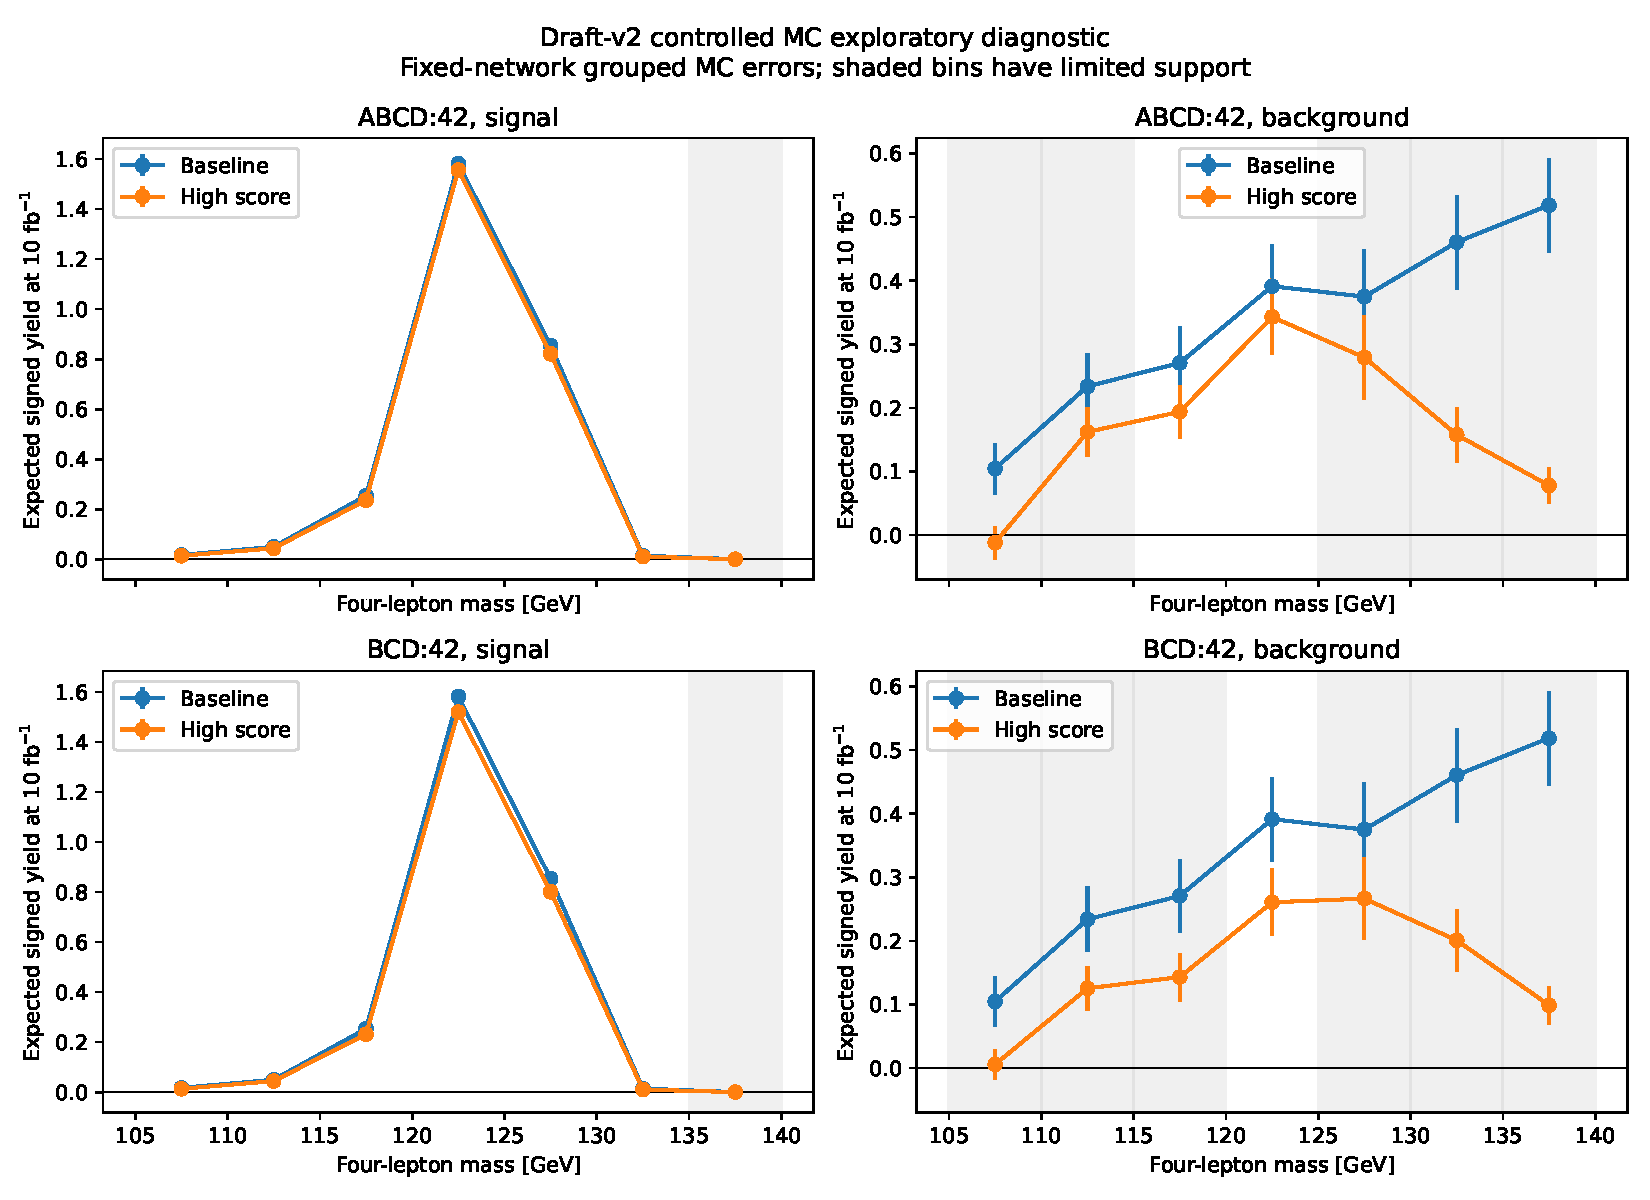
\includegraphics[width=\linewidth]{figures/draft001/mass-yields.pdf}
\caption{Signed mass spectra from draft001 final evaluation. ABCD is shown above
and BCD below, both at seed 42. Blue circles show the baseline; orange diamonds
show high-score events. Signal is left and background right. Each point represents
a 5 GeV bin; connecting lines guide the eye, not a continuous mass model. The
vertical axes report expected yields at $10\,\mathrm{fb}^{-1}$ and have different
scales for signal and background. Error bars use grouped MC variance. Shaded
regions flag limited support under the criteria below; negative yields are retained.}
\label{fig:yields}
\end{figure}

\textbf{Support flags.} A mass bin is shaded if either its baseline or high-score
sample has no event groups, nonpositive signed yield $Y$ or grouped variance $V$,
signed effective count $N_{\rm eff}=Y^2/V<20$, or cancellation ratio
$\rho=|Y|/\sum_i|w_i|<0.2$. Here $w_i$ is an event's evaluation yield weight,
and $V$ sums squared yield contributions over physical event groups. Shading
marks a support diagnostic, not a confidence band. The same criteria apply
to the normalized shapes in Figure~\ref{fig:shapes}.

\textbf{Signal location.} The simulated signal is concentrated around 125 GeV.
The two selected curves largely retain that region. The network does not move
individual event masses; any distribution change results from choosing a subset
of the baseline events. The coarse bins do not establish a peak-position shift,
an improved detector resolution or a change in the physical Higgs width.

\textbf{Background appearance.} The background extends across the mass window
and is already nonuniform before the cut. It is reduced unevenly across mass,
particularly in the upper tail. A visual increase in signal prominence therefore
needs two explanations: how much background is removed, and how the remaining
background is distributed. The separately normalized plots on the next page
address the second question.

\clearpage
\reportsection{6. How do the shapes change?}
Figure~\ref{fig:shapes} normalizes each process and selection by its own signed
total. This removes the overall yield change from the comparison. Table~\ref{tab:fractions}
quantifies the main visible changes using the same fixed mass regions.

\begin{figure}[h!]
\centering
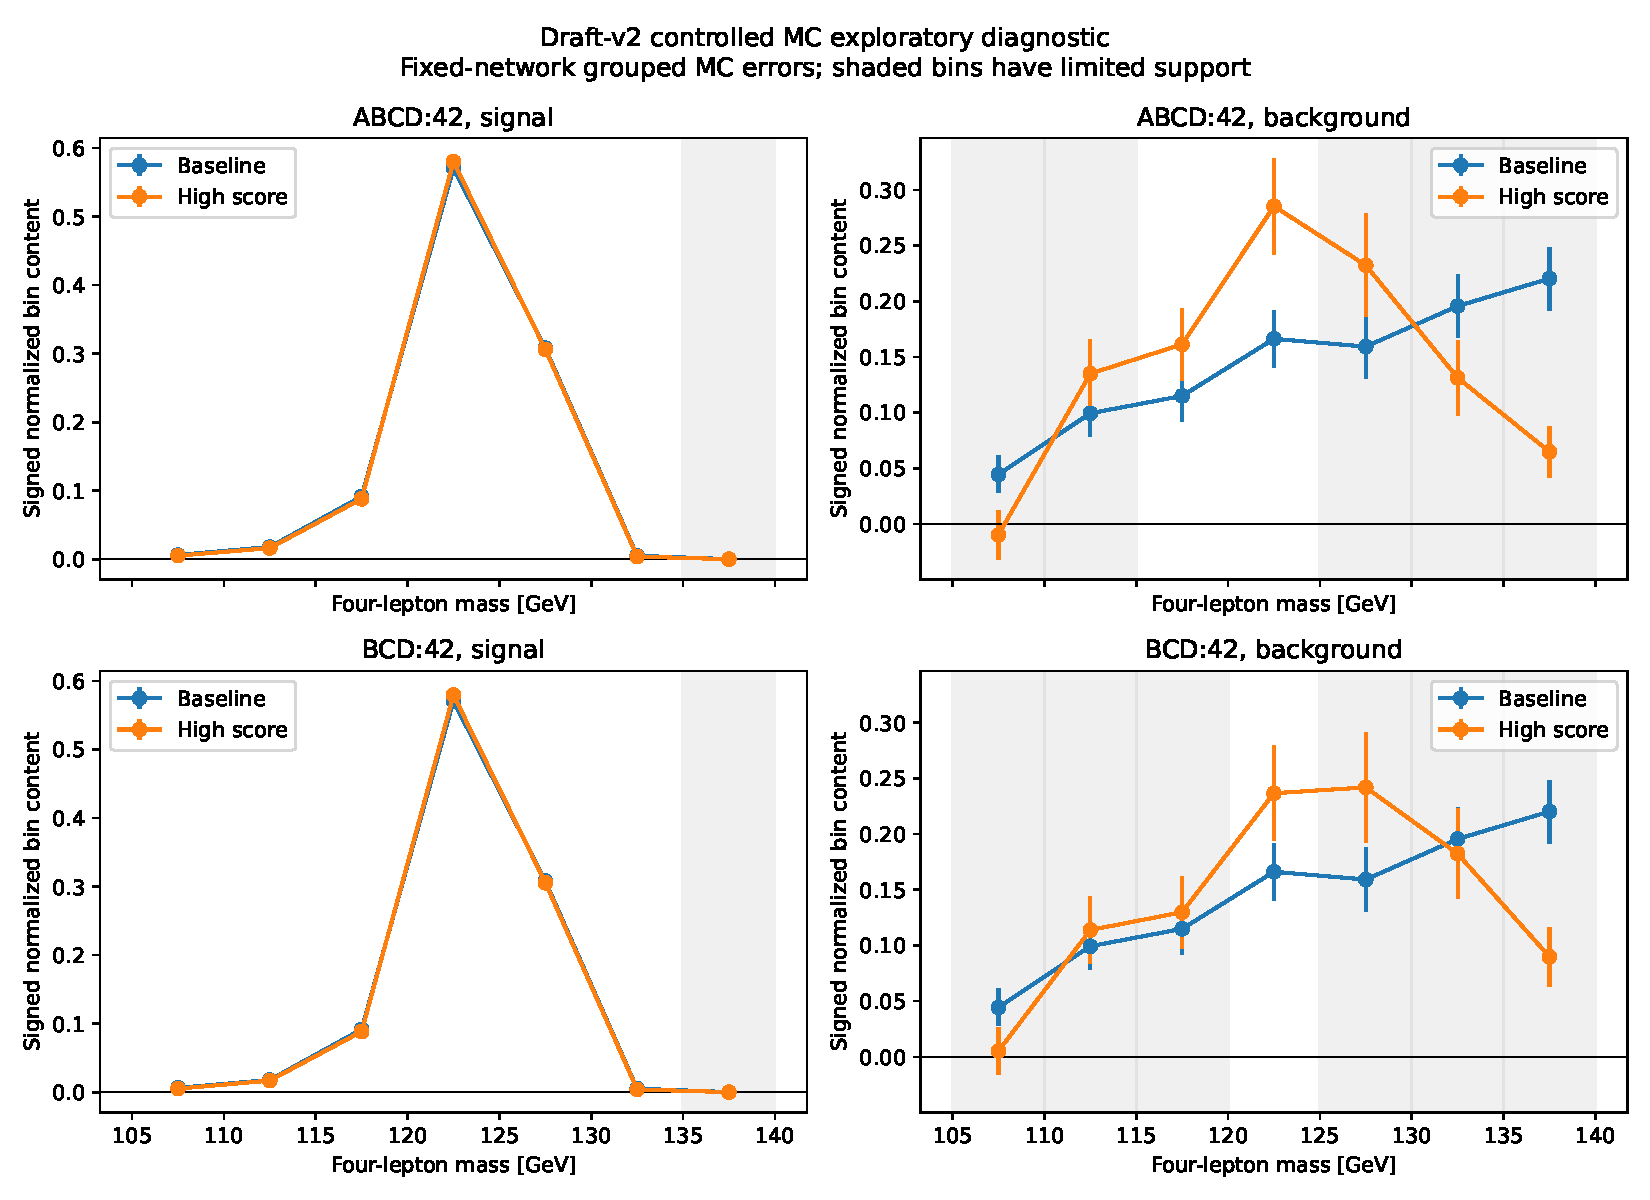
\includegraphics[width=.94\linewidth]{figures/draft001/mass-shapes.pdf}
\caption{Separately normalized before/after mass shapes for the same events and
cuts as Figure~\ref{fig:yields}. Each bin is divided by its curve's own positive
signed total. Error bars propagate shared normalization; before/after values
also share events. A signed normalized shape need not be a probability density.
Shaded and negative bins are retained without smoothing, clipping or rebinning.}
\label{fig:shapes}
\end{figure}

\begin{table}[h!]
\caption{Fraction of each curve's signed yield in fixed mass regions (\%).
Entries are descriptive point estimates; uncertainties are not displayed.
They do not establish the statistical significance of before/after differences.}
\label{tab:fractions}
\centering
\small
\begin{tabular}{llrrr}
\toprule
Process & Region (GeV) & Before & ABCD high & BCD high \\
\midrule
Signal & $[120,130)$ & 87.9 & 88.6 & 88.5 \\
Background & $[120,130)$ & 32.5 & 51.8 & 47.9 \\
Background & $[135,140)$ & 22.0 & 6.5 & 9.0 \\
\bottomrule
\end{tabular}
\end{table}

\textbf{Interpretation.} Signal remains concentrated in its main mass region.
Background becomes relatively more concentrated there, while its high-mass tail
fraction falls. This is descriptive evidence that the frozen selections depend
on mass despite omitting explicit $m_{4\ell}$. It does not identify a unique
responsible feature or establish a physical background resonance.

\textbf{Limits.} The selected ABCD background bin $[105,110)$ GeV is negative;
several background bins and the signal upper tail have low support. Shared-event
and normalization correlations prevent treating plotted errors as independent
measurements. The errors condition on fixed networks and cuts; they exclude
threshold estimation, independent retraining and coverage uncertainty.

\clearpage
\reportsection{7. Project status and next steps}
\textbf{Completed.} The simplified study trained five representations
(ABCD, BCD, ACD, ABD and ABC) for seeds 42, 43 and 44. Groups A/B/C/D describe,
respectively, individual-lepton kinematics, dilepton masses/separations,
collective-event kinematics and five angles. Every reduced model was trained
separately. All fifteen nominal intervals and the one shared inclusive-count
reference have valid numerical status.

The main metric remains $W_{68}=\mu_{\rm upper}-\mu_{\rm lower}$, the nominal
68\% signal-strength interval width under the specified model. Signal strength
$\mu$ scales the expected signal yield. Each interval uses model-self Asimov
expected observations at injected $\mu=1$, with the T1 likelihood profiling
finite-template-statistics nuisance parameters. Its endpoints use the asymptotic
68\% quantile of $\chi^2$ with one degree of freedom for the profile-likelihood
ratio statistic, within $0\leq\mu\leq20$. The nominal 68\% label does not establish
calibrated repeated-sample coverage. Both high- and low-score categories enter
the likelihood, each integrated over one mass interval, $[105,140)$ GeV.
The seven display bins in the spectra are not likelihood bins. The high-score
illustration therefore does not imply that low-score events were discarded
from inference.

\begin{table}[h!]
\caption{Compact progress summary of the nominal interval comparison.
Medians summarize three fixed training seeds, not repeated independent MC samples.}
\label{tab:widths}
\centering
\begin{tabular}{llr}
\toprule
Representation & Input group omitted & Median $W_{68}$ \\
\midrule
ABCD & None & 1.464392 \\
BCD & A & 1.474847 \\
ACD & B & 1.467509 \\
ABD & C & 1.505681 \\
ABC & D & 1.452977 \\
Inclusive-count reference & No trained classifier & 1.638845 \\
\bottomrule
\end{tabular}
\end{table}

The four comparisons are formed within each seed as
$\Delta W_G=W_{68}(\mathrm{ABCD}\setminus G)-W_{68}(\mathrm{ABCD})$, then
summarized. Removing C widens the interval for all three seeds, with median
$\Delta W_C=0.046283$. The A, B and D differences change sign across seeds.
ABC has the smallest median width among these five representations, but that
does not establish a universally optimal input set or a confirmed precision gain.

\textbf{Interpretation status.} These are exploratory, non-independent MC
results. Previously used source events remain in the study even after a new
split. The intervals use their own templates as expected observations; coverage
has not been independently calibrated. T1 accounts for finite-template statistics
within the likelihood, but does not supply complete MC uncertainty on differences
between model widths. Seed variation is not a confidence interval. The project
is an educational and technical study, not an official ATLAS/CMS result, a Higgs
discovery or a physics measurement.

\textbf{Next steps.}
\begin{itemize}
\item Review whether the before/after comparisons fully explain the selected signal and background.
\item Assess the documented project adaptations and prioritize the unresolved selection references.
\item Prioritize validation of physical weight/selection applicability, finite-MC
uncertainty of width differences and interval coverage. These remain outstanding work.
\end{itemize}

\clearpage
\reportsection{Sources and a short traceability note}
The external sources below were checked on 30 October 2026. The published
analyses provide selection context, not numerical results for this report.
The CERN record explicitly describes its collection as educational and not
suited for scientific publications. This progress report retains an
educational/technical scope; using the collection does not reproduce the
research-grade analyses cited below.

\begingroup
\small
\renewcommand{\refname}{References used in this report}
\begin{thebibliography}{9}
\bibitem{OpenData}
ATLAS Collaboration, \emph{ATLAS 13 TeV samples collection at least four leptons
(electron or muon), for 2020 Open Data release} (2020).
\href{https://opendata.cern.ch/record/15005}{CERN Open Data record 15005},
\href{https://doi.org/10.7483/OPENDATA.ATLAS.2Y1T.TLGL}{doi:10.7483/OPENDATA.ATLAS.2Y1T.TLGL}.
Source for the two simulated dataset members; see its usage statement.

\bibitem{ATLAS13}
ATLAS Collaboration, \emph{Measurement of the Higgs boson coupling properties in
the $H\to ZZ^*\to4\ell$ decay channel at $\sqrt{s}=13$ TeV with the ATLAS detector},
JHEP \textbf{03} (2018) 095.
\href{https://doi.org/10.1007/JHEP03(2018)095}{doi:10.1007/JHEP03(2018)095};
\href{https://arxiv.org/pdf/1712.02304v2#page=8}{arXiv:1712.02304v2, Secs.~5.1--5.2, pp.~8--9}.
Selection and working-point comparisons in Sections 2--3 of this report.

\bibitem{HZZCuts}
ATLAS Open Data outreach tools, \emph{HZZCuts.py}, revision
\nolinkurl{8ad2015be6d350060c3a183aff5802570bc9ada4}.
\href{https://github.com/atlas-outreach-data-tools/atlas-outreach-Python-uproot-framework-13tev/blob/8ad2015be6d350060c3a183aff5802570bc9ada4/HZZCuts.py#L2-L33}{Fixed-version source, lines 2--33}.
Multiplicity/charge, partial momentum cuts, flavour and optional isolation definitions.

\bibitem{HZZAnalysis}
ATLAS Open Data outreach tools, \emph{HZZAnalysis.py}, same revision as
Ref.~\cite{HZZCuts}.
\href{https://github.com/atlas-outreach-data-tools/atlas-outreach-Python-uproot-framework-13tev/blob/8ad2015be6d350060c3a183aff5802570bc9ada4/HZZAnalysis.py#L140-L168}{Fixed-version source, lines 140--168}.
Event-weight factors, applied cuts and commented-out isolation calls.

\bibitem{ATLASRun1}
ATLAS Collaboration, \emph{Measurements of Higgs boson production and couplings
in the four-lepton channel in $pp$ collisions at center-of-mass energies of
7 and 8 TeV with the ATLAS detector}, Phys.~Rev.~D \textbf{91}, 012006 (2015).
\href{https://doi.org/10.1103/PhysRevD.91.012006}{doi:10.1103/PhysRevD.91.012006};
\href{https://arxiv.org/pdf/1408.5191v3#page=7}{arXiv:1408.5191v3, Sec.~5.1, printed pp.~6--7}.
Reference for the trigger-matching principle; its detailed thresholds and
working points are not asserted to be this project's prescription.
\end{thebibliography}
\endgroup

\textbf{Local result source.} All numerical results and both figures come from
\nolinkurl{runs/h4l-draft-v2-draft001/report/}, linked to the completed prepare,
freeze and evaluation artifacts. Report file sizes and SHA-256 values were
checked against its manifest; both figure copies match the report byte for byte.
The detailed identity record is \nolinkurl{paper/draft-v2/DRAFT001-EVIDENCE.md}.
The frozen protocol is \nolinkurl{config/protocols/h4l_draft_v2.json}.

\textbf{Selection implementation.} Exact inequalities were checked against
\nolinkurl{config/protocols/h4l_selection_v1.yaml} and
\nolinkurl{src/higgsml/physics/selection.py}, with the draft-v2 protocol's
$[105,140)$ GeV override and $2e2\mu$ restriction. Report preparation used
completed aggregates and public documents; it did not reopen event payloads,
train models, rescore events or refit intervals. Missing step-by-step counts
remain missing rather than being estimated from another run.

\end{document}
